\documentclass{article}

\usepackage[english]{babel}

% Set page size and margins
\usepackage[a4paper,top=2cm,bottom=2cm,left=3cm,right=3cm,marginparwidth=1.75cm]{geometry}

% Useful packages
\usepackage{amsmath}
\usepackage{graphicx}
\usepackage[colorlinks=true, allcolors=blue]{hyperref}
\usepackage{subcaption}

\title{Stress Prediction from Physiological Data}


\begin{document}
\maketitle

\begin{table}[h]
    \centering
    \begin{tabular}{ll}
        Registration number: & \textcolor{red}{2201312}\\
        Link to GitHub: & \url{https://github.com/shaejaz/university-trial-analysis}\\
    \end{tabular}
\end{table}


\begin{table}[h]
    \centering
    \begin{tabular}{lc}
        Executive summary (max.\ 200 words) & \textcolor{red}{145}\\
        Main findings and Discussion (max.\ 600 words) & \textcolor{red}{585}\\
        Conclusions (max.\ 300 words) & \textcolor{red}{248}\\
        \hline
        Total word count & \textcolor{red}{978}\\
    \end{tabular}
    %\caption{Word counts for each section.}
\end{table}


\tableofcontents

\clearpage


\begin{abstract}
This report presents the findings of training and testing models to be able to predict if a user is stressed given physiological data collected by a sensor \cite{iqbal22}. The data includes heart rate, skin temperature, accelerometer data, etc. Being able to predict stress would provide much more measurable indicators of discomfort and agitation in medical patients as well as free medical staff from manually monitoring stress indicators. Some common machine learning models excel in predicting the temporal and seasonal nature of time-series data similar to our scenario. With these models, we were able to achieve moderate success in trying to predict a patient's stress. This provides promising results for not only the value and validity of the underlying data being trained on but also how even simple models can obtain worthwhile results and is encouraging further enhancements and advancement in these types of models and datasets.
\end{abstract}

\section{Main Findings}

\subsection{Overview}
For this report, three models were used and their performance was evaluated on the dataset. A basic Logistic Regression model as a base model for evaluation. The other two models are LSTM models, one being a simple single-layered LSTM and the other being a multi-layered one with Dropout layers in-between.

Splitting of the dataset was done based on different subjects. For example, subjects 1, 4, 5, and 6 were used as training sets and 2, 3, and 7 as the validation sets. This is instead of using a time-based split that is also commonly used, mostly when subject-wise divisions in the dataset are not available.

\subsection{Initial findings}
Initial evaluations of all three models were done to get a ballpark of the estimated performance relative to each other. The findings can be found below.

\ref{fig:basic_lstm_log_reg} shows that the basic LSTM model only showed marginal gains over the base Logistic Regression model, that too with possible favorable conditions.

\ref{fig:lstm_dropout_log_reg} shows that the double-layered LSTM showed slightly worse performance compared to the Logistic Regression model.

\begin{figure}[h]
\centering
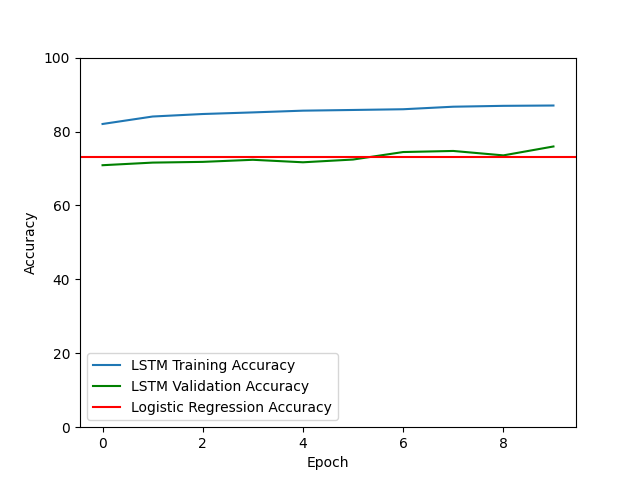
\includegraphics[width=0.3\textwidth]{report/basic_lstm_log_reg.png}
\caption{\label{fig:basic_lstm_log_reg}Results of the basic LSTM model compared to Logistic Regression}
\end{figure}

\begin{figure}[h]
\centering
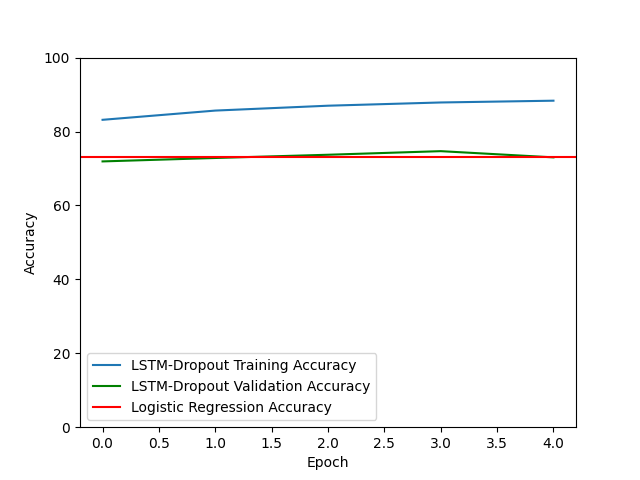
\includegraphics[width=0.3\textwidth]{report/lstm_dropout_log_reg.png}
\caption{\label{fig:lstm_dropout_log_reg}Results of the double-layered LSTM-Dropout model compared to Logistic Regression}
\end{figure}

\subsection{Cross-validation}
Cross-validation was performed on all three models to get more robust and accurate performance metrics. This was done using a 5-fold split of the subjects. The results of the cross-validation training are in table \ref{tab:crossvalidation}.

\begin{table}[h]
\centering
\begin{tabular}{l|r}
Model & Average Accuracy (\%) \\\hline
Logistic Regression & 73.67 \\
Basic LSTM & 74.53 \\
Double-layered LSTM and Dropout & 73.76
\end{tabular}
\caption{\label{tab:crossvalidation}Cross-validation accuracy.}
\end{table}

All results are very close to each other, with the basic LSTM taking a very slight edge. 

\subsection{Dropping doubtful features}
This section overviews how the removal of certain columns/features affect the performance of a model. As the previous sections have highlighted that all models are close to each other in terms of performance, we will use one model here, Logistic Regression.

The results of these actions of the training data are presented in table \ref{tab:droppedcolumns}.

\begin{table}[h]
\centering
\begin{tabular}{l|r}
Dropped Columns & Average Accuracy (\%) \\\hline
'X', 'Y' and 'Z' & 73.34 \\
BVP & 75.10
\end{tabular}
\caption{\label{tab:droppedcolumns}Dropped features accuracy.}
\end{table}

These columns were chosen as they have the most erratic distribution of values over time. The results seem to support that this nature of these features do not contribute much to the data.

\section{Discussion}
From the above results, there are a few key insights that we can gather about the data and the methodology. First, we observed next to no improvement upon a basic Logistic Regression model when switching over to a more advanced LSTM network. This was both in the case of a very simple LSTM network and one with more layers.

We can make a few deductions based on this data. It might suggest that the underlying data in its current form might not be suitable for LSTM and the RNN family of models. There might be a need to explore some additional data pre-processing techniques especially those specific to time-series data. Other model architectures might also be needed to be investigated at the same time that are distinct from LSTMs.

It might also be possible that this data simply requires much bigger LSTM models with more layers than the ones used in this report. LSTM layers take a long time to train and this requirement could result in much greater costs than expected for the company.

It might be that the data is lacking in terms of useful features that are needed when stress needs to be predicted. This is supported by the fact that dropping some of the columns results in a non-significant change in the average accuracy of the models. There might be a need to get additional sensors and replace them with the ones producing not as useful data.


\subsection{Limitations}
The main limitation of the current approach is that only LSTMs (in turn RNNs) have been explored in this report. Moreover, due to the cost of training the LSTM layers, the models were of relatively small size


\section{Conclusions}
We can see that the models used in training on the dataset can produce satisfactory results, although it is important to note that in a high-risk environment such as the treatment of patients by medical professionals, the performance of the models needs to be much higher. This requires a large amount of refinement on the data collection, both in terms of process and data features being gathered. The models that have been used in this report also have certain lacking characteristics, specifically in terms of layers and complexity. 

There are also some changes to the techniques incorporated in the methodology that can be modified. A viable experiment would be to use a different cross-validation method. Instead of folding on the subjects, a more traditional time-series folding approach can be taken such as training only on certain contiguous parts of the dataset after combining all data from the subjects into one. The cross-validation approach in this report can then be compared and its performance tradeoffs analyzed.

As stated in the beginning, this report and findings only deal with the prediction of stress not forecasting. Forecasting requires a different set of models currently being presented but is a valid and obvious future extension of the findings. Using the common and cutting-edge models in the forecasting space such as ARIMA, SARIMAX and Prophet \cite{prophet23} (forecasting model created by Meta) can lead to even further use cases for the project as medical professionals will gain an entirely new data point when treating patients.

\bibliographystyle{abbrv}
\bibliography{main}

\end{document}